\subsection{Remote vs Local Library} \label{sec:remoteVsLocal}

\begin{figure}
    \centering
    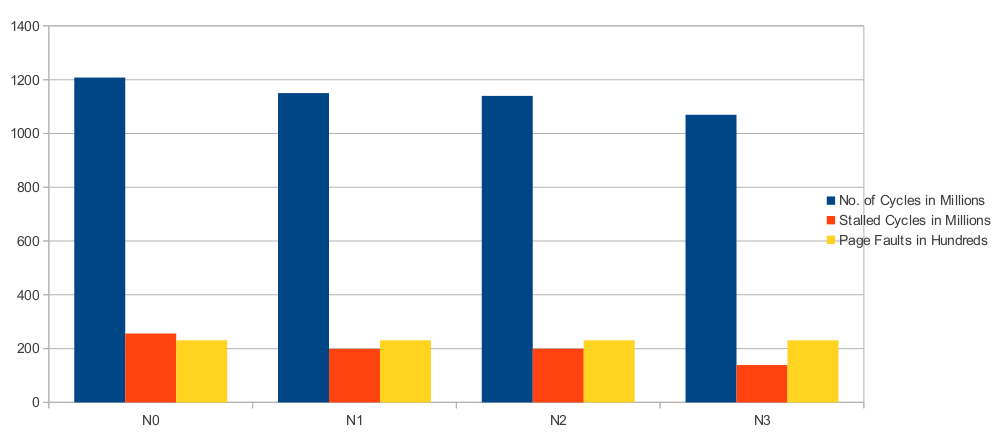
\includegraphics[scale=0.35]{remoteVsLocal.png}
    \caption{Comparision of remote vs local library. N0, N1, N2, N3 are nodes in NUMA machine. Shared library is at N3 }
    \label{fig:remoteVsLocal}
\end{figure}


In the above section we saw the interconnect overhead in terms of slowdown in time when data is fetched from remote node.
Similar overhead exist in the case when read-only data is being fetched from remote node \cite{Drepper07whatevery}.
We tried to see that slowdown in the case of shared libraries, which are also the read-only data.
The shared library was placed on node N3.
Then we wrote a main thread which called functions from this shared library.
We ran the main thread on each of the four nodes (N0,N1,N2,N3).
Main thread called 0.1 million functions from the library in sequential order.
Figure \ref{fig:remoteVsLocal} shows the result.
We measured the total number of CPU cycles consumed, stalled cycles and page faults in each case.
We observed that in the case when our main thread was running locally (i.e. on node N3), it consumed minimum number of CPU cycles.
Number of stalled cycles were also minimum when library is placed locally, high number of stalled cycles in remote case indicates that lot of CPU cycles were idle due slow for data fetch over the interconnect.
We measured page faults to make sure that we are fetching equal number of library pages in all four cases, and number of page faults were equal in all four cases.
The number of cycles consumed were proportional to the interconnect slowdown we saw in above section.
From the slowdown Matrix in figure \ref{fig:numaMatrix} we see that N0 is farthest to N3, hence maximum cycles are consumed by node N0 and least for the local node.



\subsection{Small vs Big functions in Library}

\begin{figure}
    \centering
    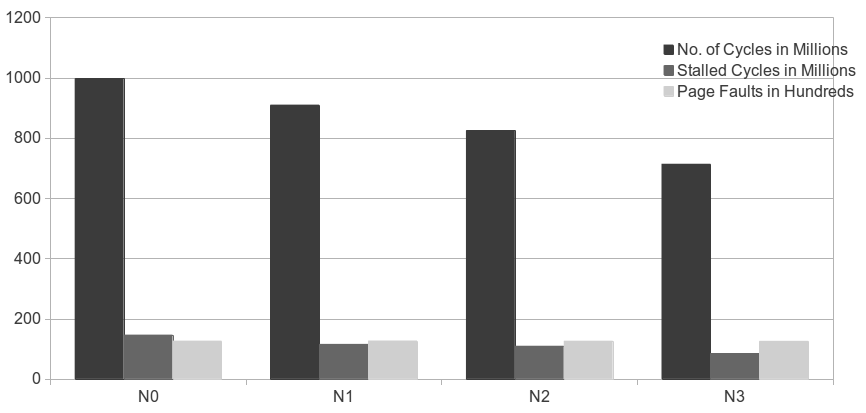
\includegraphics[scale=0.35]{smallFunc.png}
    \caption{Performance with small sized functions. Shared library is at N3 }
    \label{fig:smallFunc}
\end{figure}

The size of each function in above section is about 600 Bytes.
We tried to make smallest possible functions which look like this:

\texttt{ int f_i()\{return i;\} }

with size of 138 Bytes for each function.
With small sized functions we wanted to see if instruction caching can help to even out the impact of remote library fetch.
Figure \ref{fig:smallFunc} shows the result.
Experimental settings were similar to section \ref{sec:remoteVsLocal}, shared library was on Node03 and we ran main thread on each of the four nodes.
The results we observed showed similar behavior as in section \ref{sec:remoteVsLocal}.
Number of CPU cycles consumed by remote nodes were more than those consumed by the local nodes, and size of the function does not matter for remote and local instruction fetching.



\subsection{Various probability distributions of function calls}

\begin{figure}
    \centering
    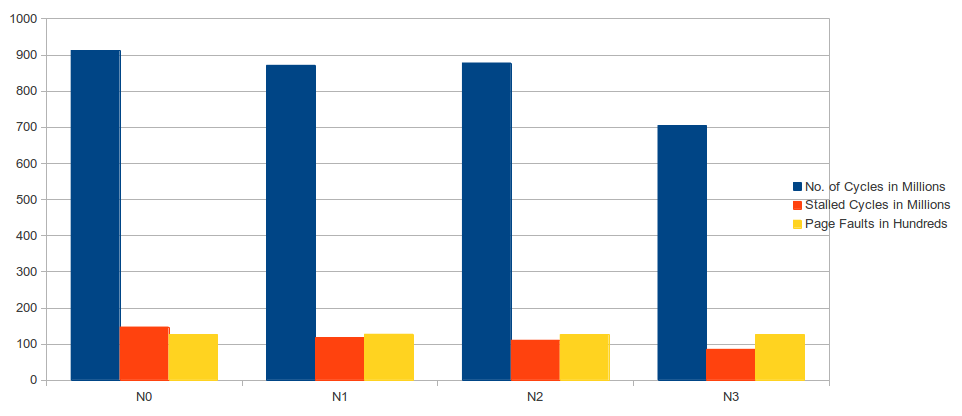
\includegraphics[scale=0.35]{randomDistribution.png}
    \caption{Library functions called in random order by main thread. Shared library is at N3 }
    \label{fig:randomDistribution}
\end{figure}

\begin{figure}
    \centering
    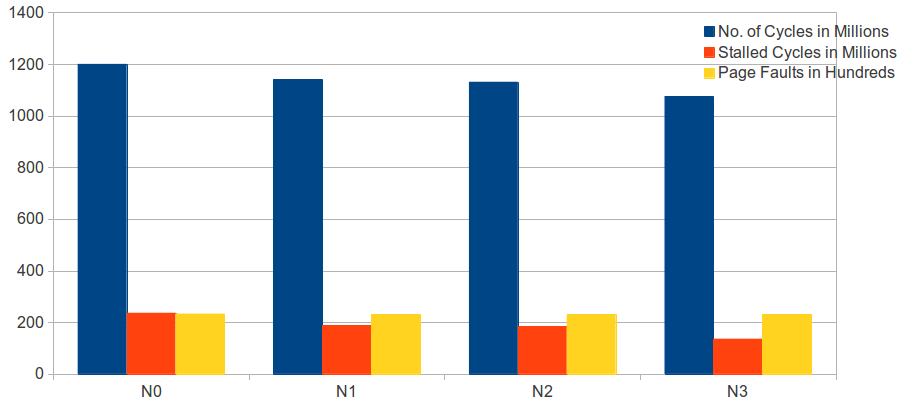
\includegraphics[scale=0.35]{zipfDistribution.png}
    \caption{Library functions called in Zipfian order (with alpha=0.5) by main thread. Shared library is at N3 }
    \label{fig:zipfDistribution}
\end{figure}

Till now we were calling the functions from the shared library in sequential order.
We wanted to vary our function calling pattern to random and zipfian distributions.
In reality it is not necessary that an application is using all the functions of a library and in sequential order.
Instruction caching favours sequential order and to negate the effect of caching we wanted to test random and zipfian distributions.

\textbf{Sequential} - Figure \ref{fig:remoteVsLocal} shows the results for sequential calling pattern

\textbf{Random} - Figure \ref{fig:randomDistribution} shows the results for calling library functions in random order.
The difference in the CPU cycles consumed by N3 (local) and N0,N1,N2 (remote) looks more pronounced.

\textbf{Zipf} - Figure \ref{fig:zipfDistribution} shows the results for calling library functions in zipfian order.
According to zipfian distribution there will be a bunch of functions which will be called more frequently than others.
Therefore instruction caching will favour the performance in this case.
Due to which the difference in the CPU cycles consumed by N3 (local) and N0,N1,N2 (remote) is not great.


\subsection{Varied Library Sizes}

\begin{figure}
    \centering
    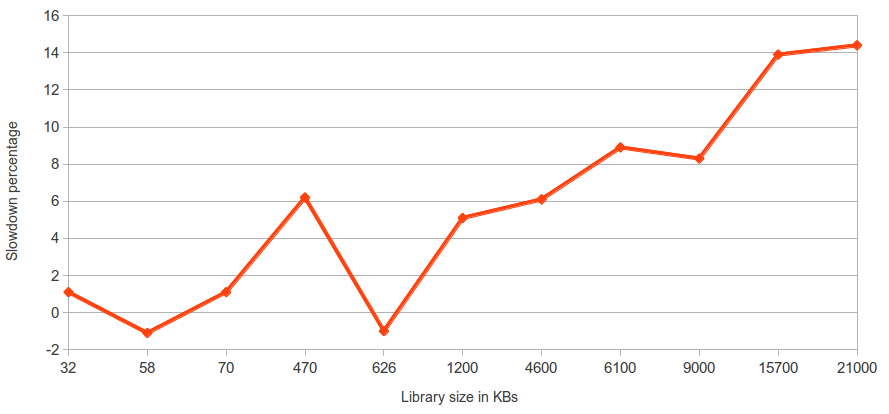
\includegraphics[scale=0.37]{slowdownWithSize.png}
    \caption{Slowdown with increasing library size }
    \label{fig:slowdownWithSize.png}
\end{figure}

Our shared library size in all the above experiments was 60MB.
In this section we will vary the size of library and find the variation in the slowdown.
We generated libraries of sizes varying from 32KB to 21MB, see Figure \ref{fig:slowdownWithSize.png}.
We kept the size of each function same at around 600 Bytes, and increased the number of functions available in each library.
When the library is small enough to fit in the cache, there won't be any instruction fetches across interconnect.
But with the increasing size of library, it will be tough to get the whole library in cache in single fetch.
Therefore library instructions will be fetched as and when needed.

The main thread calls the library functions in sequential order.
And number of calls made by the main thread is equale to the number of functions available in the library.
For example, our 32KB library had 50 functions and main thread made 50 calls.
Reason behind not doing equale number of calls for all the libraries was to avoid the page fault factor in CPU cycles measured.
Lets say we do one million calls for a library with ten thousand functions, some functions will be called repeatedly in cyclic order and will cause page faults.
Setup was very much similar to above experiments, we had our library on one node and main thread ran on all the four nodes.
We then measure the CPU cycles consumed by local and remote node for each library.
The ratio of CPU cycles consumed by remote node over local node gave us the slowdown.

The result is shown in Figure \ref{fig:slowdownWithSize.png}.
We observed that when the library is small enough to fit in the cache, not much slowdown is observed.
It has even gone to negative in some cases.
But as the size of library increases and instructions are fetched over interconnect, we see that the slowdown has increased.
It is 14\% for 21MB library.
